


\begin{figure}[h!]%h!
    \centering
    \begin{subfigure}{.47\textwidth}
        \centering
        %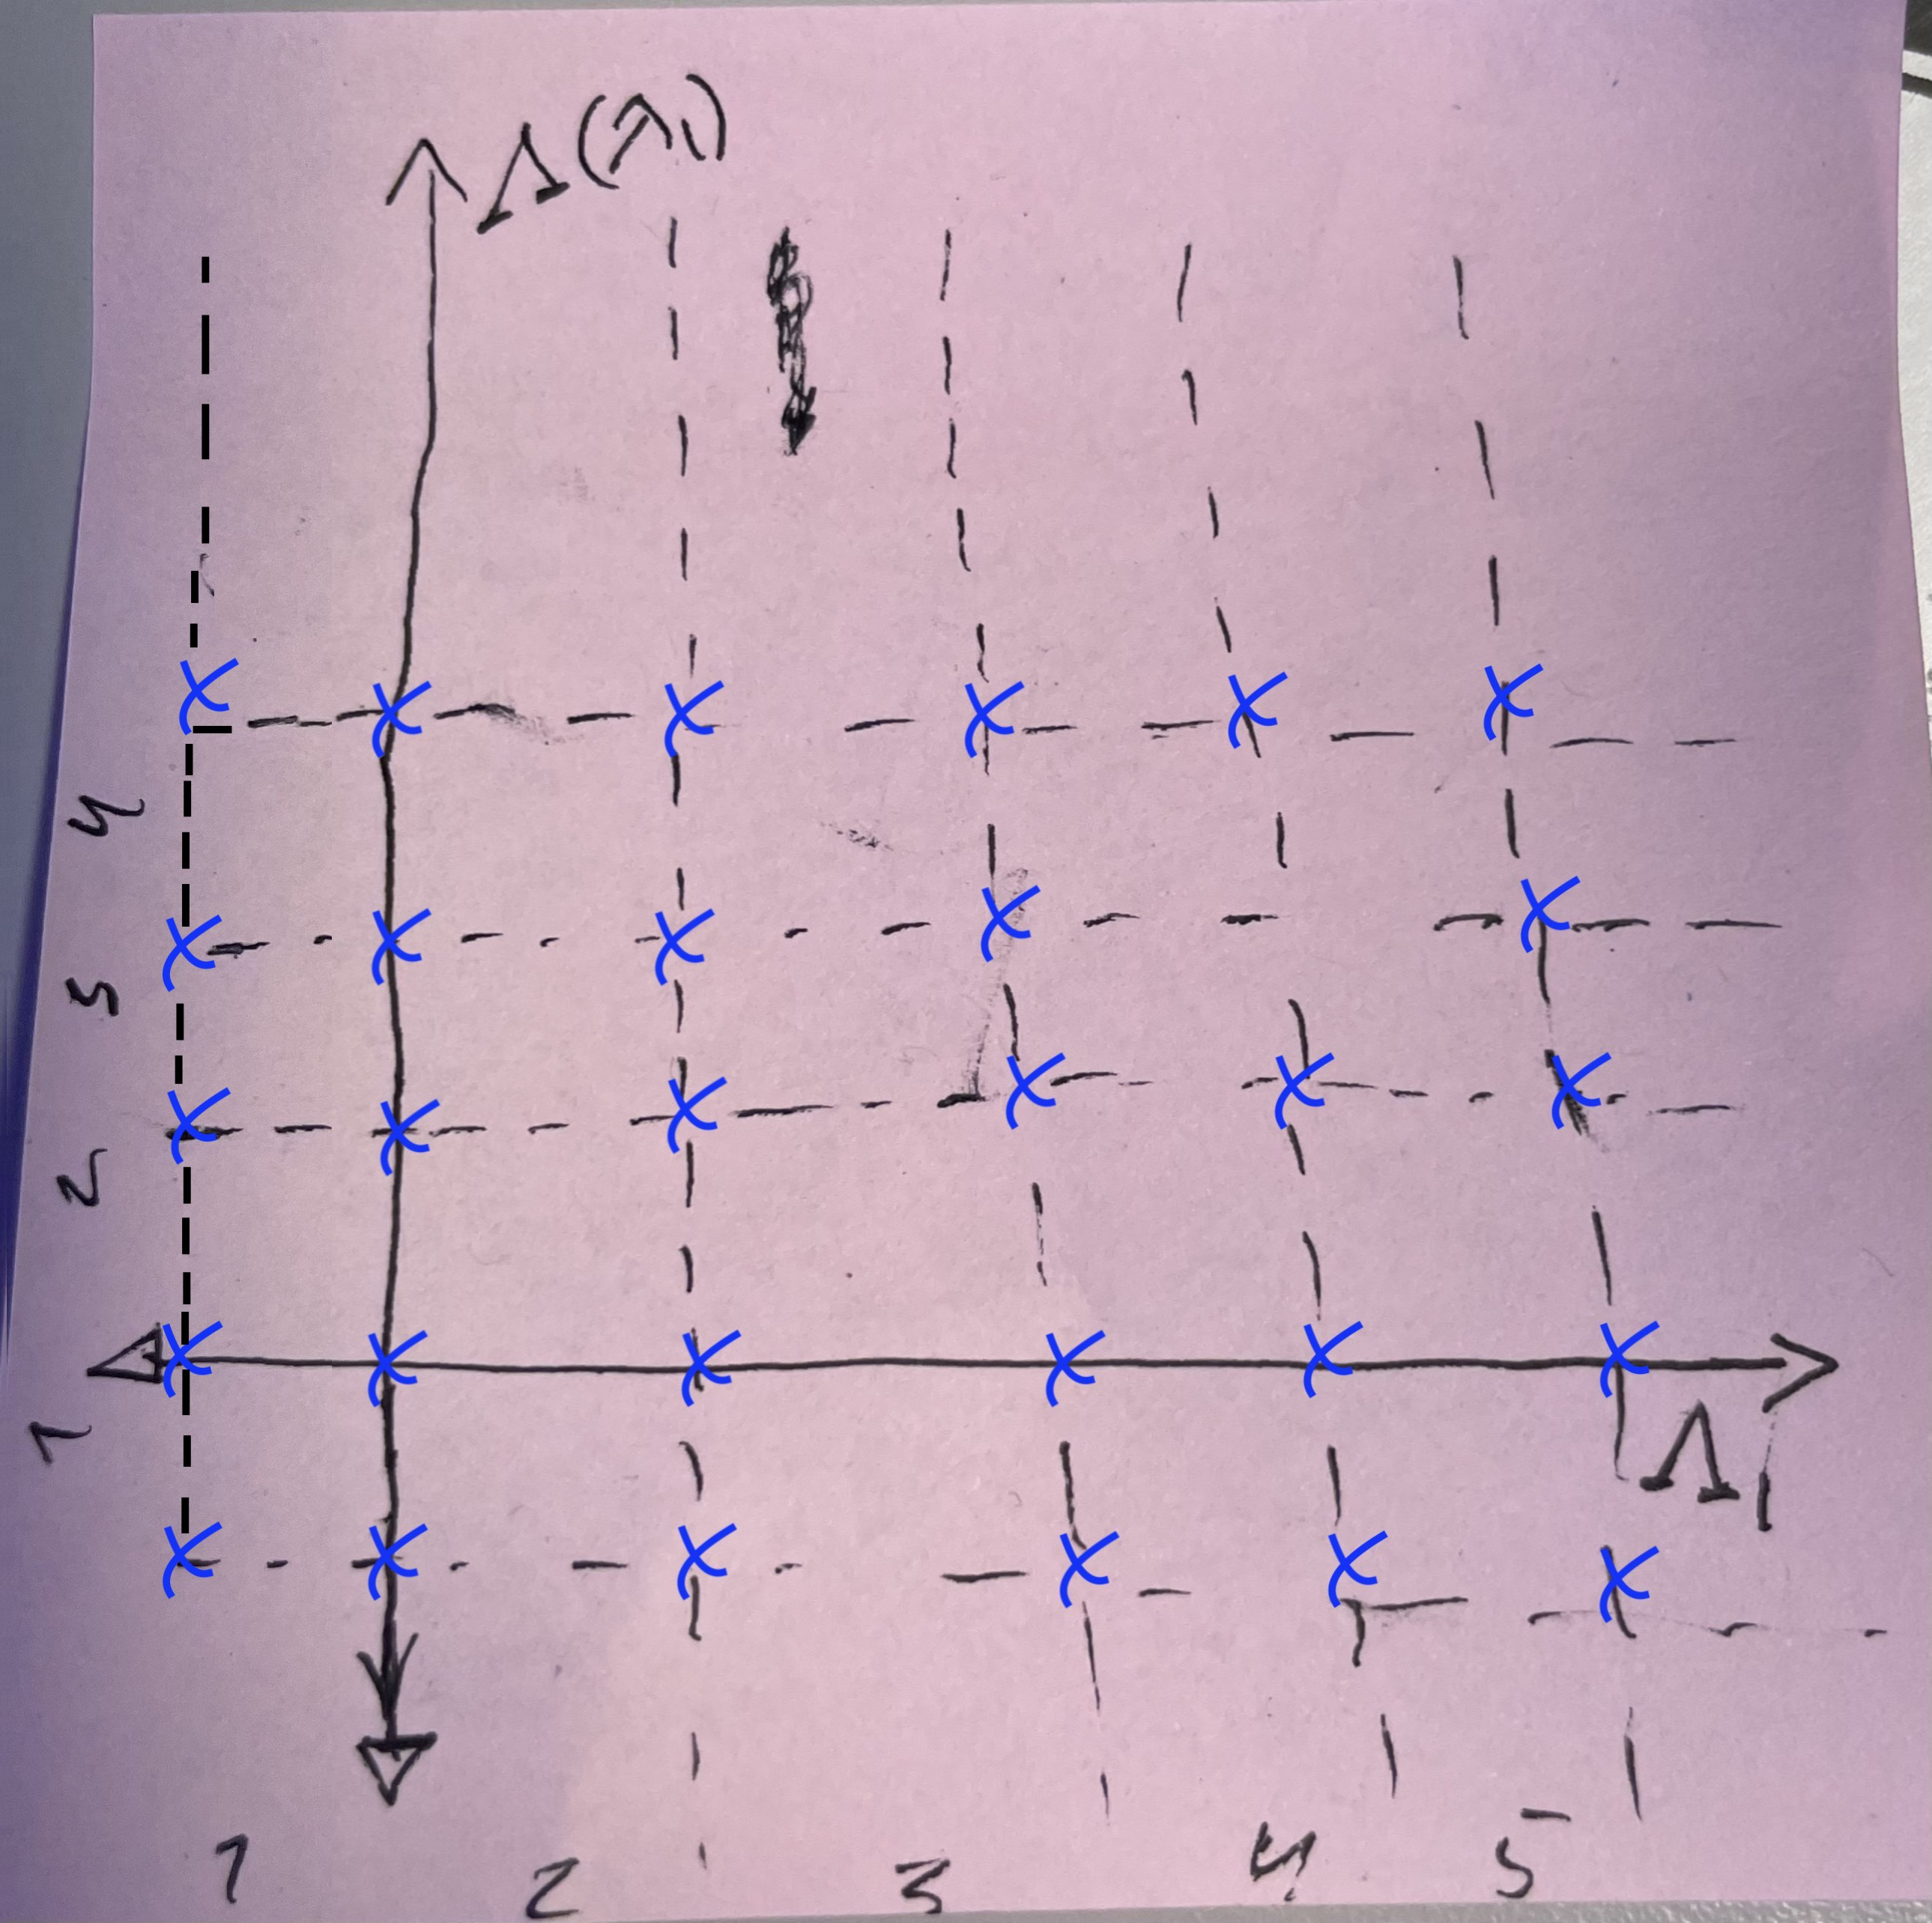
\includegraphics[width=0.9\linewidth]{spec_no_shift.jpg}
        %* Figure 1
        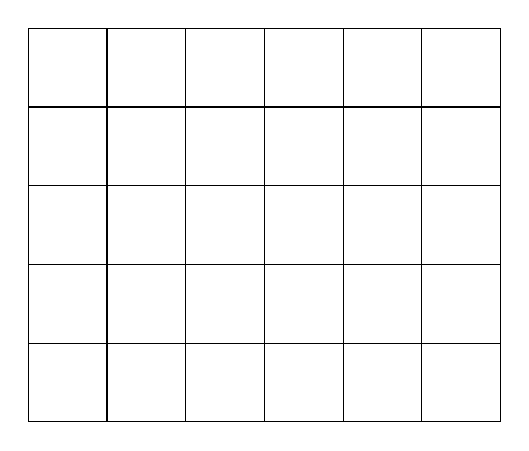
\begin{tikzpicture}[scale=1]
            % Define the tile
            \def\tile{
              % Draw the unit square
              \draw (0,0) rectangle (1,1);
            }
          
            % Draw the tiling pattern
            \foreach \x in {0,1,2,3,4,5}{
              \foreach \y in {0,1,2,3,4}{
                \pgfmathsetmacro{\shiftX}{\x} % Set horizontal shift
                \pgfmathsetmacro{\shiftY}{\y} % Set vertical shift
                \begin{scope}[shift={(\shiftX,\shiftY)}]
                  \tile % Draw the tile
                \end{scope}
              }
            }
        \end{tikzpicture}
        %* —————————————————
        \caption{Lattice spectra}
        \label{fig:tiling_one}
    \end{subfigure}\quad
    \begin{subfigure}{.47\textwidth}
        \centering
        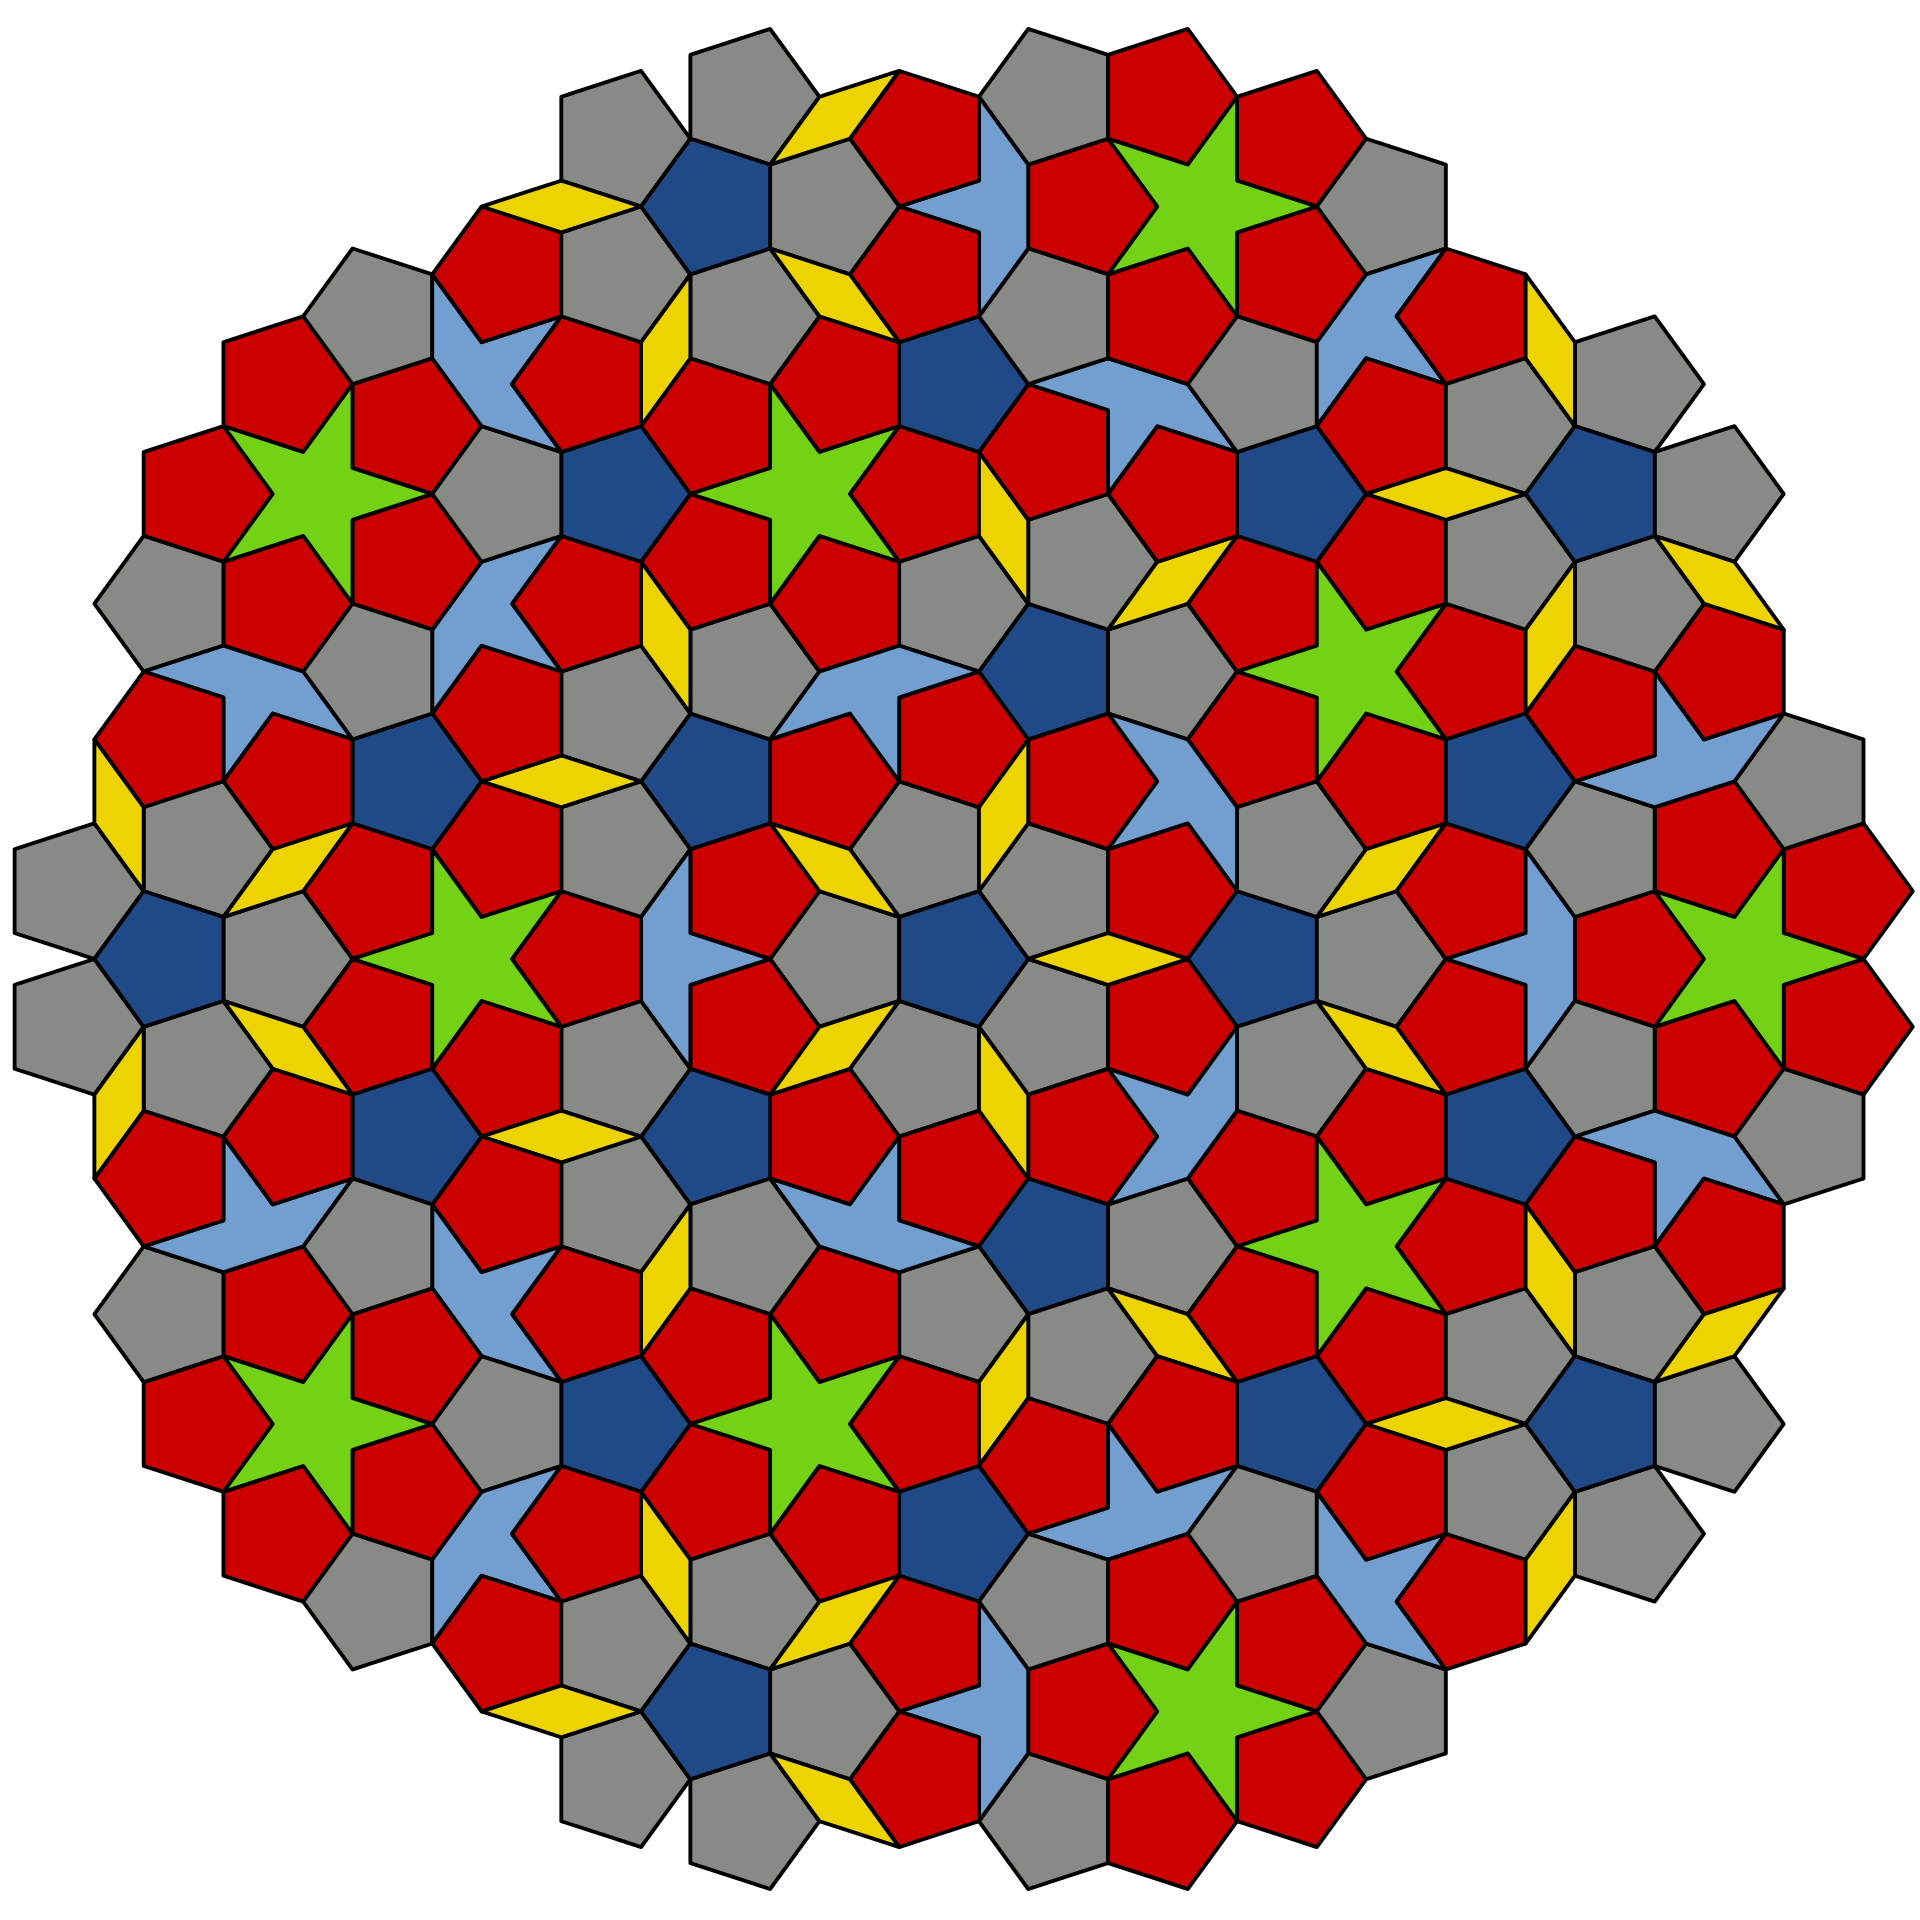
\includegraphics[width=0.9\linewidth]{Penrose_Tiling_.png}
        \caption{P1 Penrose Tiling}
        \label{fig:tiling_two}
    \end{subfigure}
    \caption{Penrose original aperiodic tiling \cite{penrosePentaplexityClassNonPeriodic1979}, from \cite{inductiveloadP1TilingUsing}, forklare fargelegginen, \SigridComment{By Inductiveload - Own work, Public Domain, https://commons.wikimedia.org/w/index.php?curid=5839133}}
    \label{fig:tilingsss}
\end{figure}
